\documentclass[../main.tex]{subfiles}

\section{Planlegging, bygging og Kontinuitet}

\subsection{Organisatorisk Kompetansebygging}
Som nevnt i innledningen er Eit-prosjektet en startfasen av et langsgående prosjekt med større rammer enn kun EiT. Av den grunn måtte vi danne en organisasjon, som skulle rekrutere flere medlemer utenfor denne Eit-gruppen og finansiere utgifter vi skulle ha ved byggingen av en ROV. 

Grunnen til at vi behover å rekrutere nye medlemmer til at vi skal rekrutere nye medlemmer er delvis for å øke den samlede kompetansen til Vortex NTNU. Delvis for å kunne øke arbeidsmengde og delvis for å bygge kontinuitet. For å rekrutere måtte vi først gjøre Vortex NTNU kjent på NTNU. Dette gjorde vi gjennom å henge opp plakater over hele Gløshaugen og å stå på stand på stripa. Vi lagde også nettside, med adresse www.vortexrov.no, for å øke legitimiteten til Vortex NTNU og for at interesserte søkere skal kunne ha et sted å finne mer innformasjon. Vi fikk inn en god del søknader og er i disse dager i prosessen med å evaluere søkerene og å ta inn nye medlemmer.

For å finansiere prosjektet trengte vi resurser. Vi beregnet i starten at vi i første omgang trengte noen titalls tusen kroner og vi behøvde derfor å bringe inn noen sponsorer. Vi satte fort i gang med å høre om noen ville sponse oss. Det første vi gjorde var å lage en liste over bedrifter vi trodde kunne ha lyst til å sponse prosjektet vårt. Disse ble valgt ut i fra om de drev med virksomheter knyttet til ROVer, nyttelast eller at de leverte produkter som vi kunne bruke til bygging av en ROV. Etter dette tok vi en ringerunde og kom i kontakt med noen bedrifter som var interessert. En av disse var Norsk Elektro Optikk (NEO). Deretter sendte vi mail til bedriftene som sa seg interessert per telefon der vi fortalte hvorfor vi ville ha dem med på laget. NEO var villig til å sponse oss, men kom også med noen oppgaver de hadde lyst på at ROVen skulle kunne utføre. Neo sponset oss med 50 000 kr. Astrup ble kontaktet angående materialer vi trengte til rammen til ROVen og de sa seg villige til å sponse disse materialene og maskinering av disse.

\subsection{Rammestruktur}
Daniel hadde ansvaret for å designe rammestrukturen, siden han var den eneste i gruppa som hadde bakgrunn innen produktutvikling og produksjon.

\subsection{CAD-modellering}

\subsection{Bygging av selve strukturen (Masse bilder)}


\subsection{Thruster}
Totalt har ROVen 8 thrustere. To er rettet oppover, to i midt seksjonen og to i hver sin ende. Ende thrusterne er vendt 45 grader inn mot hverandre for å gi mer bevegelses muligheter til ROVen.
 
Notasjonen som er brukt angående retninger til ROV er i henhold til SNAME notasjonen \cite{fossen}.
 
Kontrollsystemet er designet som en PID kontroller i surge, hive og jaw.. Kontrolleren er laget slik at det er enkelt å gjøre endringer. Valg av integralvirkning er problematisk hvis en ikke tar hensyn til at motorene kan gå i metning. Løsningen der er å ha to tilstander i regulatoren. Går motoren i metning skal integratorene kobles ut slik at de ikke bygger seg opp.
 
Vi har valgt å ikke ha styring for sway roll og pitch. Plassering av thruster muliggjør ikke styring for roll. Her har vi antatt at den roven vil være naturlig stabil, slik at små rullebevegelser som vil forekomme vil bli rettet opp av roven uten hjelp fra thrustere.

\subsection{Kontroll av kraft til thrusterne}
 
ROVen er et overaktuert system, noe som gjør at det ikke eksisterer en unik løsning for kraft fra hver enkelt thruster. For å løse problemet optimal med individuell styring av alle thrusterne blir problemet et lineært problem \cite{opti} med 8 variabler og tre ligninger. Utvider vi problemet til å ta utgangspunkt i at thrusterne kan gå i metning får vi 16 variabler og tre ligninger. For å løse dette problemet trenger vi en kraftigere microkontroller, siden vi mistenker at den kontrolleren vi har ikke vil oppfylle et real time demand som trengs for et styresystem. Problemet er løst med dele de forskjellige thrusterne inn i grupper. De to øverste funger som en enhet, og fokusere kun på hive. De to bakerst styres individuelt, mens de fire fremst fungerer som støtte motorer når de bakerste går i metning. 

\subsection{System arkitektur}
 
Vi har valgt å skrive i tre forskjellige programmeringsspråk. Styresystemet er skrevet i C++, mens kommunikasjonen er skrevet i Python. I tillegg er seriell kommunikasjon mellom Raspberry Pi og Arduino skrevet med et sett av C/C++ funksjoner, som tar hånd om prototyper og andre små endringer før det oversettes til C++. Systemet har et modulisert design, slik at deler skal enkelt bli erstattet i fremtiden. Topside løsningen vår er at vi har en PC, og i ROVen har vi en Rasberry Pi og en Arduino Mega 2560.

\subsection{Laser Shark}
Payloaden ble bestemt at skulle være NEO sin Laser Shark da dette var et krav fra NEO som nevnt tidligere. En Laser Shark består primært av en linjelaser og et kamera plassert med ca 2m innbyrdes avstad. Formålet med dette utstyret er å lyse på havbunnen med laseren for så å lage en avblidning av havbunnen ved hjelp av kameraet. 
For oss førte dette med seg endel desing valg og utfordringer. Vi måtte først og fremst ha flere typer spenninger, da laseren går på 48 V og kameraet går på 24 V i tillegg trenger laseren en kjølepumpe som etter spesifikasjonene går på 12 V. Så var det den fysiske størrelsen på ROVen, denne måtte ta høyde for at kameraet og laseren trengte en innbyrdes avstand av ca 2 m. Et siste krav fra NEO var at ROVen skulle kunne holde en stabil rettning med en hastighet på 0.5 m/s.

\subsection{Elektronikk}


\subsection{Oppdriftelement}
Oppdriften til ROV-en skal balanseres ved hjelp av et oppdriftselement lagd av Divinycell. Divinycell er et skummateriale laget av en blanding av polyurea og pvc. Leverandøren Diabgroup anbefaler H130 som oppdriftselement til ROVer som skal ned til 75 m under havet. H130 skal ha en kompresiv styrke på 2,4 til 3,0 MPa noe som betyr at det skal tåle trykk ned på over 2 bar.

Tettheten til sjøvann er $1,025 g/cm^3$. Divinycell H130 har en tetthet på 0,130 $g/cm^3$ \cite{seawater}. Dette gir en netto oppdriftskraft tilsvarende 0,895 kg per liter oppdriftselement.

Oppdriftselementene blir kjøpt som plater med dimensjonene $1960 \cdot 970 \cdot 30 mm^3$. Disse vil blir skjært til ved hjelp av en CNC maskin og limt sammen med en epoxyblanding. I tillegg skal den bli coatet med epoxy blandet med et pigment som skal gi gul farge.


\subsection{Elektronikkbokser}

Kravet for elektronikkbokser er at hver av dem skal inneholde en strømforsyning med målene $295 \cdot 127 \cdot 41 mm^3$, en strømforsyning med målene 78 x 51 x 28 mm, 4 Electronic speed Controllere til thrusterne og kabler for å koble elektronikken sammen. I tillegg har strømforsyningene vifter som skal hjelpe til å kjøle dem ned.  For at disse ikke skal blokeres lager vi boksen litt større enn strømforsyningene. Vi valgte å lage 2 bokser med målene $450 \cdot 150  \cdot 150 mm^3$. Da dette er mer en nokk til å få plass til det som skal være opp i. I tillegg kan vi få plass til flere ting hvis vi velger å utvide ROVens funksjonalitet.

Boksene er laget av aluminium. Hovedgrunnen til dette er på grunn av aluminiums gode varmeledningsevne. Strømforsyningene i boksen har en makseffekt på omtrent 1000 W og en effektivitet på omtrent 80 \%. Da kan vi anslå at det blir dannet 200 w varme når motorene er på maks effekt som gir 100 w per boks. Siden vi ikke har oversikt over strømningsforholdene i boksen, er det vanskelig å finne ut elektronikken blir nok avkjølt. Hvis vi antar noen verdier for konveksjon og antar at veggene oppfører seg som en plate med areal lik summen av arealet til alle veggene og at kjølesystemet i strømforsyningene veldig effektivt, kan vi regne ut varmeoverføring med en temperaturforskjell på $40 \degreeC$ mellom havet og elektronikken:
 
\begin{equation} \label{eq:1}
q = \frac{\Delta T}{\frac{1}{h_luft}+\frac{\Delta x}{k}+\frac{1}{h_{vann}}}= 400 W/m^2 
\end{equation}

\begin{equation} \label{eq:2}
A_{tot} =0,2925 
\end{equation}

\begin{equation} \label{eq:3}
Q=A_{tot} \cdot q= 117 W
\end{equation}

Overslaget gjort i ligning \eqref{eq:1}, \eqref{eq:2} og \eqref{eq:3} viser at boksen greier å transportere ut mer varme en det som blir dannet med full effekt på motorene når temperaturforskjellen er $40 \degreeC$. Tallene er hentet fra tabell \ref{t:nyttig}. Siden motorene bare går på full effekt i små tidsrom og beregningene ikke tar for seg direkte konduksjon fra elektronikken til aluminiumboksen, kan vi si at vi er på den sikre siden, selv om vi tar veldig mange antakelser i utregningen med tanke på konveksjonskonstanter og form.\\
 
Elektronikkboksen skal tåle å være på en dybde på 100 m under havet. Dette gir et trykk på 10 bar. Med modellering i Comsol som vist i Figur \ref{f:sim}, ser vi at maks spenning en aluminiumboks med veggtykkelse på 10 mm vil oppleve er 6,24 MPa. Aluminiu 6061 T6 har en flytespenning på minst 241 MPa og sveist 6061 har flytespenning på 75 MPa \cite{6061}. Vi vil derfor unngå flyt i alt for stor grad på 100 m under havet.
 
% MÅ KNYTTES INN!
\begin{table}
	\caption{Nyttige verdier}
		  \label{t:nyttig}
	\begin{tabular}{ l r }
	Egenskap & verdi \\ \hline
	Termisk ledningsevne aluminium & 237 W/(m K) \cite{Aluminium} \\ 
	konveksjon vann & ~$50 W/(M^2 K)$\cite{mit} \\ 
	konveksjon luft & ~$10 W/(M^2 K)$ \cite{mit} \\ 
	 
	\end{tabular}
\end{table}

\begin{figure}[h!]
    \centering
    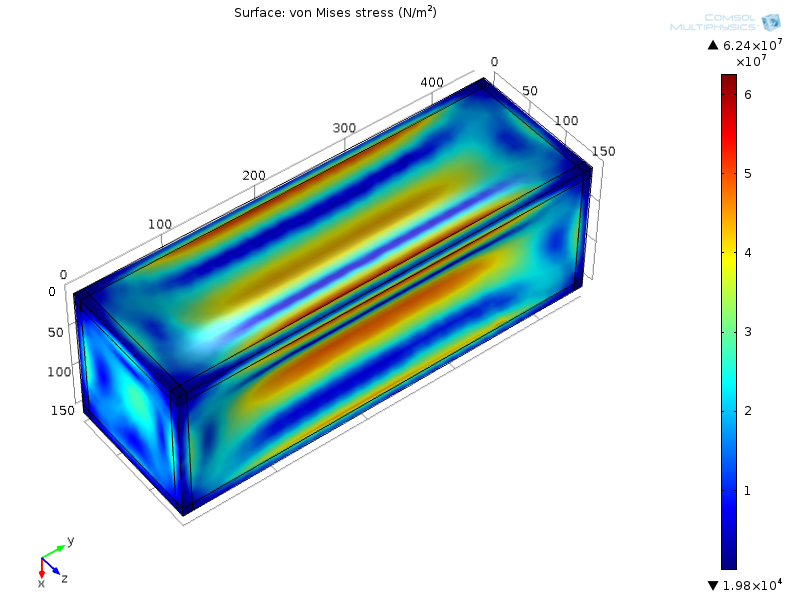
\includegraphics[width=0.4\textwidth]{img/simulering.png}
    \caption{Simulert spenning i aluminiumsboks ved 10 bar trykk (ca 100 m)}
    \label{f:sim}
\end{figure}
